Meshroom is a free, open-source 3D reconstruction software developed by AliceVision. The main way of using it is by connecting nodes which compute data. To start, open Meshroom, select File$\rightarrow$New Pipeline$\rightarrow$Photogrammetry, drag and drop the images of the object you want to reconstruct into the image gallery and press start. After the nodes have finished computing you can double click on them to view their results. 

\subsection{Nodes}

\subsubsection{CameraInit}
    This node processes the given pictures into data that Meshroom can use. It also reads the metadata from the pictures to acquire information that can be used later in the pipeline for example the focal length or the intrinsic parameters of the camera.


\subsubsection{FeatureExtraction}
    This node extracts distinct points from the images called features. In its parameters we can specify which method we can use. The default and a lot of the times the best method is dspsift(domain size pooling scale invariant feature transform), but there is also the akaze method which can be used for challenging surfaces like skin. Here we can also specify to extract points with cctags which we can use to scale the finished model by specifying the real world positions of those tags(Note: if using cctags, every picture must have at least 1 visible cctag and the pictures should be scaled down to something like 1920x1080 because it has a MAX\_RESOLUTION limit hard coded).
    In the settings of this node we can also give masks for the pictures so it only extracts points in a given field on the image. We can also change how much and the quality of the extracted points.
    
\subsubsection{ImageMatching}
    This node matches images so we know which images are close by so we can use them later for the FeatureMatching. There are multiple methods of ImageMatching. VocabularyTree sorting and comparing the extracted features of every image. Sequential matches images based on their name. Exhaustive matches every image with every image. Frustum matches based on the known image poses and matches images that are close by. 

\subsubsection{FeatureMatching}
    This node goes through the found image pairs and it finds similar features on both images. In the settings there is a parameter called minimal 2D motion. By default it is -1, meaning disabled, but if we put it to some positive value, like 2, we specify that a point to be matches, it needs to not be in the same position in both images. This option is useful to filter out background matches if we use turn tables because the background is static.

\subsubsection{StructureFromMotion}
    This node uses those matches features and uses that data to give us the position of those points in 3D space and the pose (position and orientation) and internal calibration of all the cameras. 

\subsubsection{PrepareDenseScene}
    This node undistorts the images. It uses the calibration parameters from the StructureFromMotion to compute the undistorted images. 

\subsubsection{DepthMap and DepthMapFilter}
    These nodes compute the depth maps of the images. The filter filters out incoherent depth map values. We can specify a downscale factor, the lower the factor is, the greater the quality, but the longer the computation time. We should use 1 only when we have very high quality images. 

\subsubsection{Meshing and MeshFiltering}
    Meshing is performed from the SfM data and the depth maps. The result is a dense geometric surface representation of the scene. This mesh then we can apply laplacian filtering to remove local defects. In the settings we can specify the output file type which we can find in the MeshroomCache folder and we can open and manipulate it with other applications like Blender.

\subsubsection{Texturing}
    This node textures the mesh. For each triangle, it uses the visibility information associated to each vertex to retrieve the texture candidates. It select the best cameras based on the resolution covering the triangle. Finally it averages the pixel values using multiple bands in the frequency domain. 

\subsection{Post processing}
    We can use an application like Blender to view and manipulate with our result mesh. Most commonly we can cut unwanted parts from our mesh, scale the mesh based on known geometry and then we can do measurements of the reconstructed object. 

\subsection{Results}
    To show the functionality of Meshroom, we will analyze the following reconstructions that i made and post-processed them in Blender.

    \subsubsection{Guitar}
    This model was made from 310 pictures from different angles. The guitar was positioned in the center of a desk and the desk was positioned in between 2 ceiling lamps so that the lighting is mostly equal from both sides. The pictures were taken by phone which i held. Because i held it and my hand isn't very stable i had to use a low shutter speed, 1/25s in these pictures, which made the pictures dark and to counter that i used a high ISO factor of 1200. I also put CCTags on the desk, but Meshroom gave me problems in scaling which i will fix in the future, and used them in Blender to scale the model. From the results we can see that a lot of my room was reconstructed from the backgrounds of the pictures, altho not in much detail. One of the things that Meshroom uses for matching is also background details, in this example that is great because every angle of the background is unique. I cut the guitar from the model in Blender. We can see that the neck of the guitar and the non glossy parts are very well reconstructed. The biggest mistake is in the body of the guitar. There is a big hole where the guitar is most glossy, that is because of the reflection of the lamps on the guitar body. In the future this can be removed by using a polarizing filter, using matte paint on the object or having better lighting. Also the pictures for this model were captured in JPG and in RAW format. The results for the reconstruction showed that JPG images were a lot better that those in RAW format. 
    
        \begin{figure}[h]
            \begin{subfigure}{.5\textwidth}
                \centering
                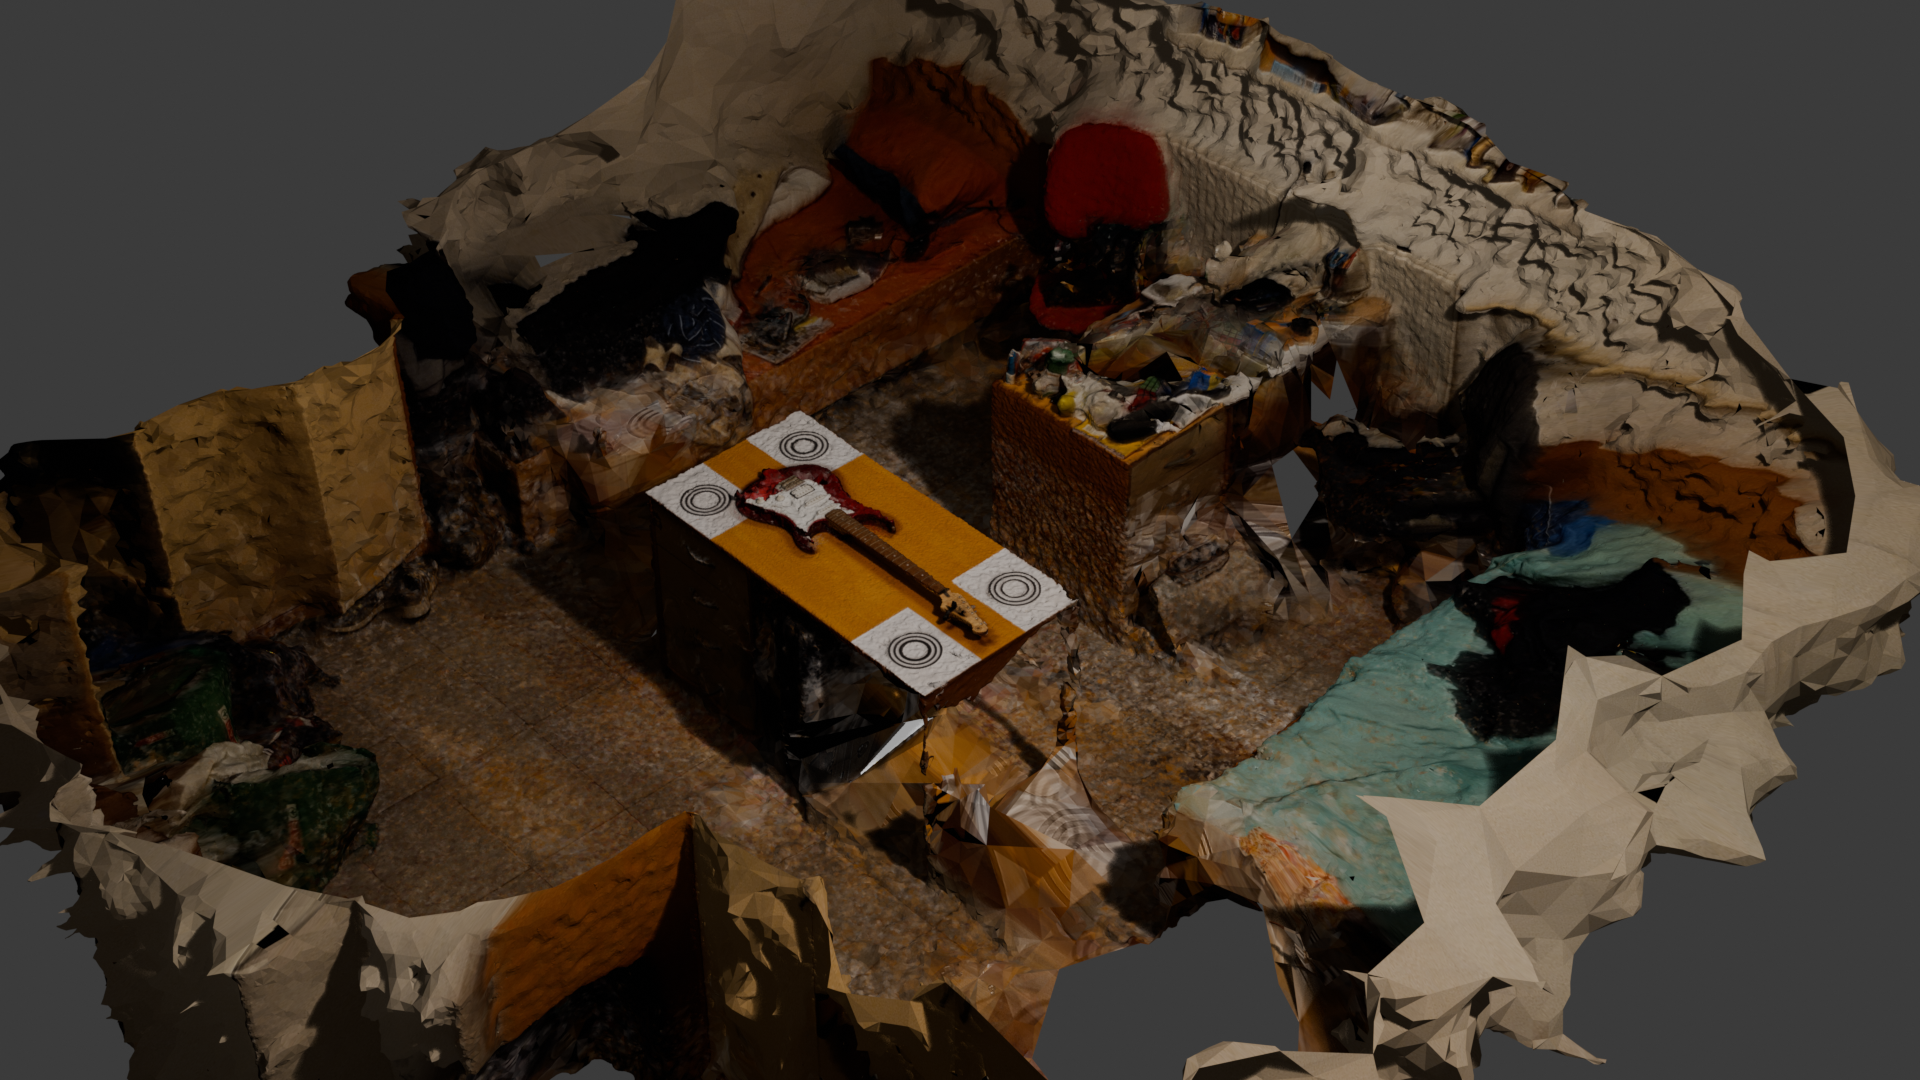
\includegraphics[width=.95\linewidth]{imgs/guitarsoba.png}
                \caption{Entire result from Meshroom}
            \end{subfigure}
            \begin{subfigure}{.5\textwidth}
                \centering
                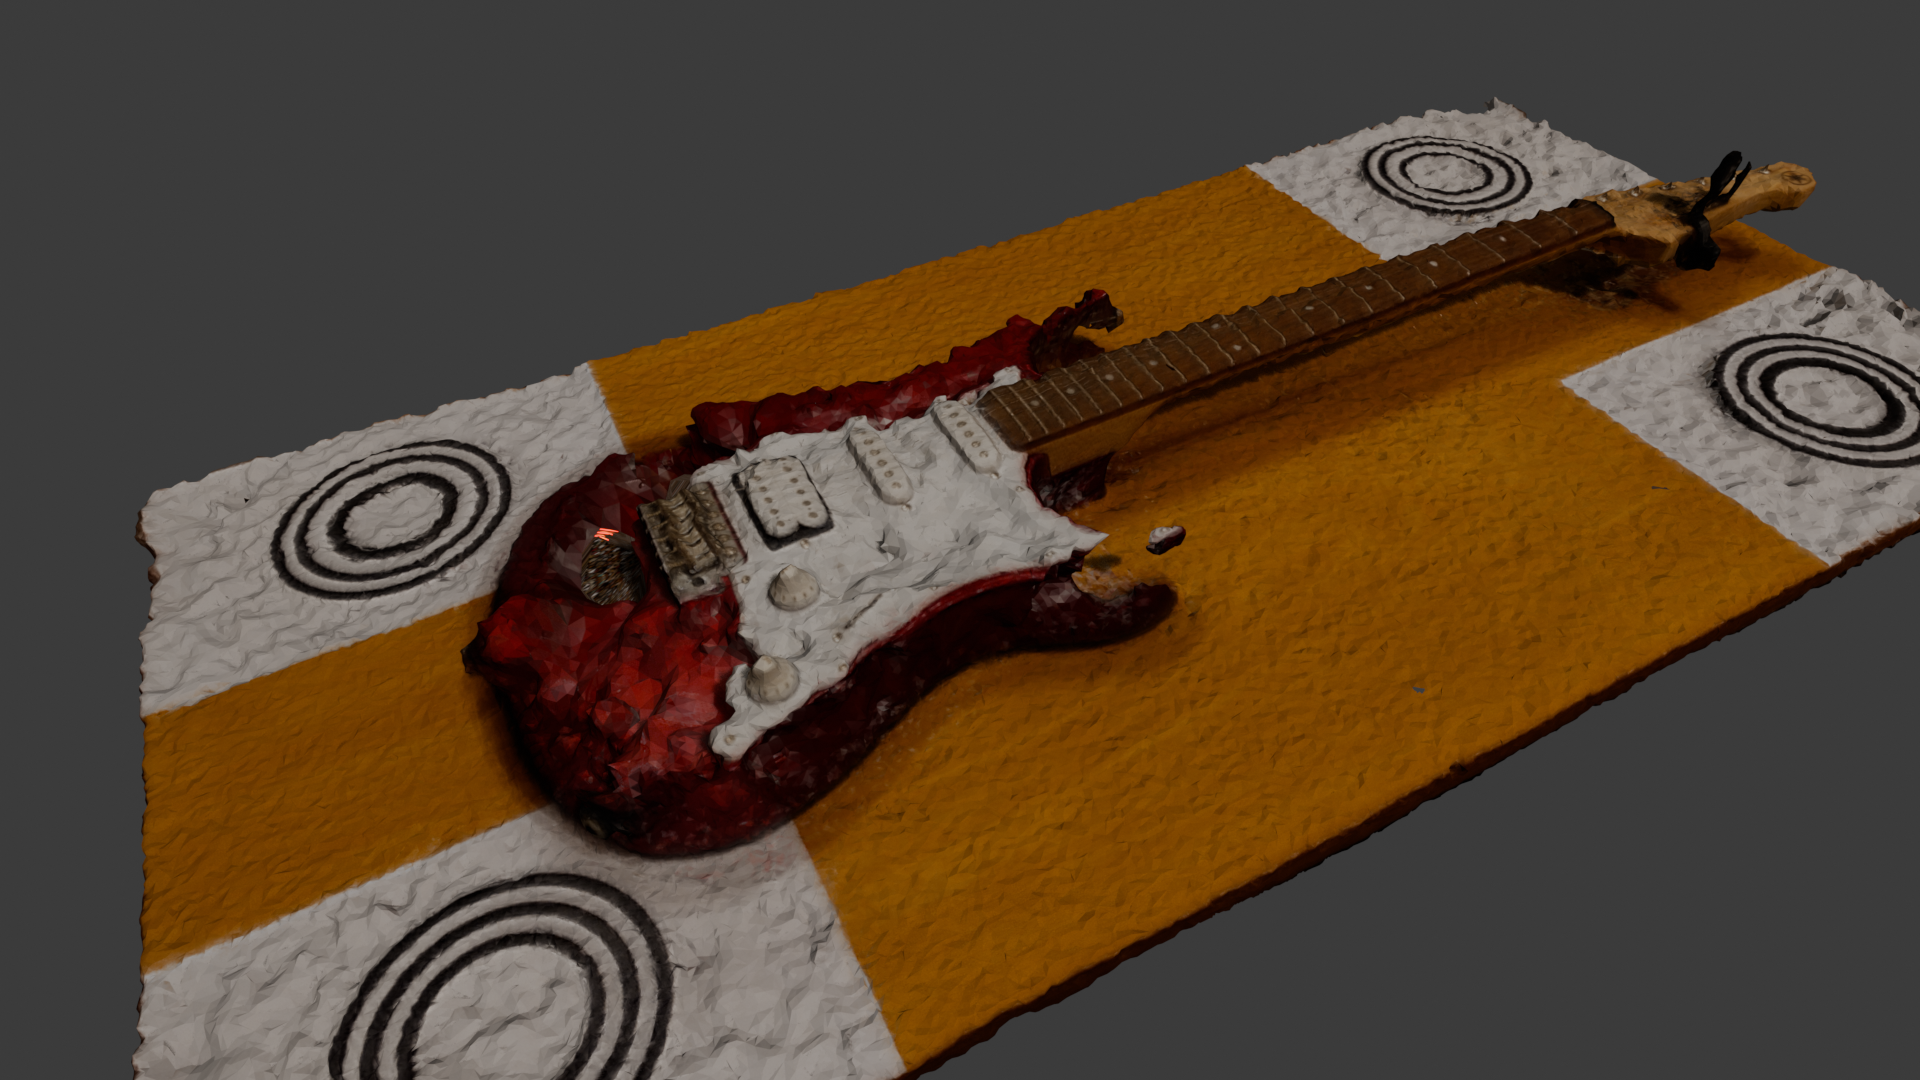
\includegraphics[width=.95\linewidth]{imgs/guitarcut.png}
                \caption{Cut result}
            \end{subfigure}
            \caption{Guitar reconstruction}
        \end{figure}
    
    \subsubsection{Eyelid}
        This model was made from 34 close up pictures of my black eye. The idea was to test how much detail can be captured on the face and the bruise. The lighting was from a desk lamp focused towards the eyelid. The shutter speed is 1/20s and the ISO is 150. The pictures were taken on a hand held phone. I did the reconstruction with different parameters so that they can be compared. The statistics on the objects can be seen in table \ref{tab:objstat}. We can see that for this example, dspsift is much better than akaze. We can also see that by having higher settings we get better results, but the difference between high and ultra is very small. From the bellow images we can notice that akaze has much more "waves" than dspsift.  

        \begin{table}[h]
            \centering
            \begin{tabular}{|c|c|c|c|c|c|} \hline 
                 &  DSPSift Normal&  DSPSift High&  DSPSift Ultra&  DSPSift+Akaze& Akaze\\ \hline 
                 Vertices&  319630&  325135&  325175&  324528& 151640\\ \hline 
                 Edges&  952816&  968875&  969452&  967321& 451475\\ \hline 
                 Faces&  635128&  645823&  646201&  644784& 300898\\ \hline
            \end{tabular}
            \caption{Object statistics}
            \label{tab:objstat}
        \end{table}

        \begin{figure}[h]
            \begin{subfigure}{.5\textwidth}
                \centering
                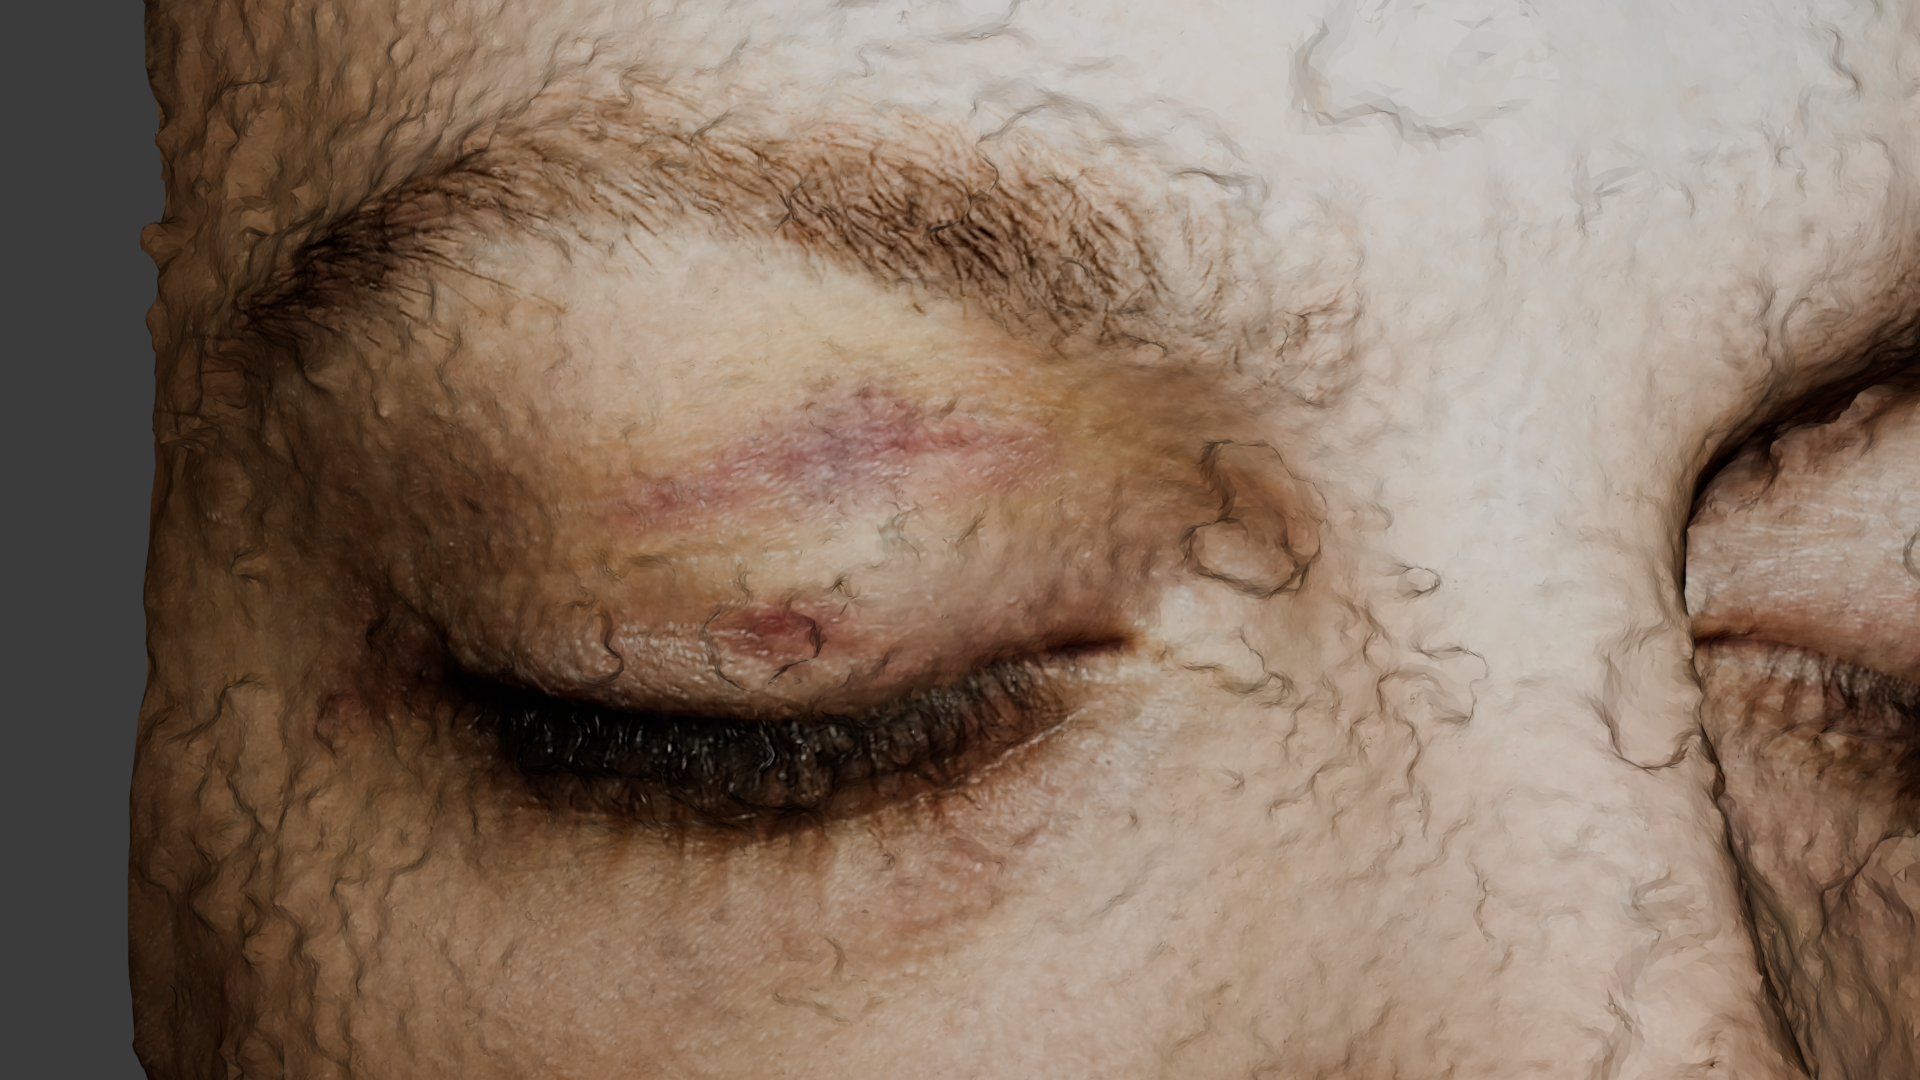
\includegraphics[width=.95\linewidth]{imgs/akaze.png}
                \caption{Akaze method}
            \end{subfigure}
            \begin{subfigure}{.5\textwidth}
                \centering
                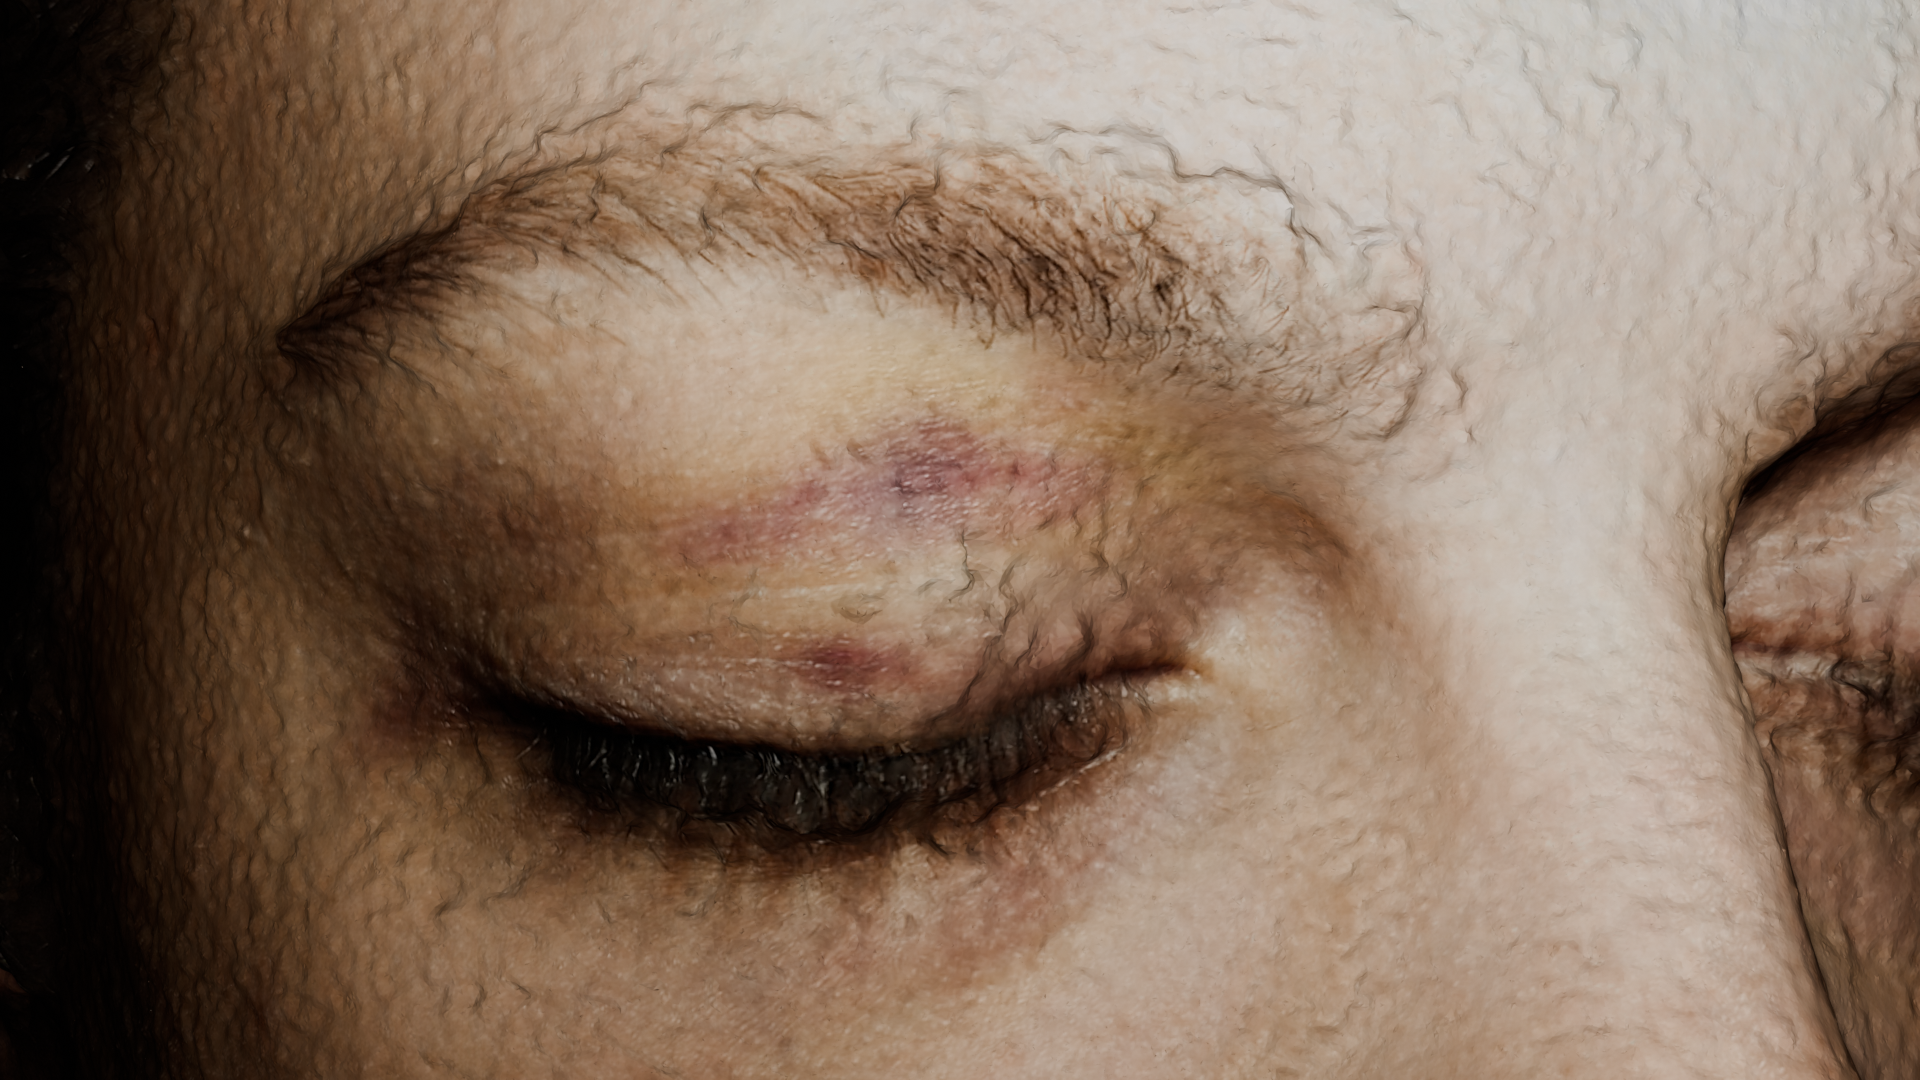
\includegraphics[width=.95\linewidth]{imgs/ultrarender.png}
                \caption{Ultra settings}
            \end{subfigure}
            \caption{Eyelid reconstruction}
        \end{figure}
    
    % \subsubsection{} %probaj parfem popravi ili arhitekt

    \subsubsection{Summary}
        For a good reconstruction we need to take good pictures. Ideally our camera should have a lower shutter speed and ISO factor. Also we should take our pictures in JPEG rather than RAW format. Lighting is very important. It should be directly on the object, not casting shadows. Out object should not be reflective because reflections of the light source give mistakes in the reconstructed model. DSPSift method for feature extraction is better than Akaze in the tested examples, but maybe for more difficult surfaces, Akaze might be appropriate. The settings on quality and quantity of extracted features should also be changed according to the number of images and the level of detail wanted. 